\documentclass[10pt]{scrartcl}

\usepackage[T1]{fontenc}
\usepackage{amssymb, amsmath, amsthm}
\usepackage{geometry, graphicx, enumitem, wrapfig, fancyhdr,cancel}
\usepackage{listings, xcolor}
\usepackage[english]{babel}

\definecolor{codegreen}{rgb}{0,0.6,0}
\definecolor{codegray}{rgb}{0.5,0.5,0.5}
\definecolor{codepurple}{rgb}{0.58,0,0.82}
\definecolor{backcolour}{rgb}{0.95,0.95,0.92}

\lstdefinestyle{mystyle}{
    backgroundcolor=\color{backcolour},   
    commentstyle=\color{codegreen},
    keywordstyle=\color{magenta},
    numberstyle=\tiny\color{codegray},
    stringstyle=\color{codepurple},
    basicstyle=\ttfamily\footnotesize,
    breakatwhitespace=false,         
    breaklines=true,                 
    captionpos=b,                    
    keepspaces=true,                 
    numbers=left,                    
    numbersep=5pt,                  
    showspaces=false,                
    showstringspaces=false,
    showtabs=false,                  
    tabsize=4
}
\lstset{style=mystyle}
\geometry{a4paper, margin=0.8in}
\pagestyle{fancy}
\lhead{PH2101 - Assignment 02 Solutions}
\rhead{Debayan Sarkar \texttt{22MS002}}
\everymath{\displaystyle}
\theoremstyle{definition}
\newtheorem{exercise}{Question}
\newenvironment{solution} {\begin{proof}[\normalfont \textbf{Solution}]} {\end{proof}}

\renewcommand{\qedsymbol}{}
\newcommand{\nn}{\mathbb{N}}
\newcommand{\npixL}{\frac{n\pi x}{L}}
\newcommand{\rn}{\mathbb{R}}
\newcommand{\q}{\mathbb{Q}}
\newcommand{\p}{\mathcal{P}}
\newcommand{\z}{\mathbb{Z}}
\newcommand{\dx}{\mathrm{d}x}
\title{PH2101 - Waves and Optics}  
\subtitle{Assignment 2 Solutions}
\author{Debayan Sarkar \\ \texttt{22MS002}}
\date{\today}

\geometry{a4paper, margin=1in}
\setlength{\parindent}{0pt}
\begin{document}
\maketitle
\begin{exercise}
    Consider a beaded string of $N$ beads each of mass $m$ (approximated as a long chain of spring-
    mass system as shown in the figure). The beads are uniformly placed on the string and the
    string has a uniform tension $T$ . The horizontal distance between any two beads in equilibrium
    is a. The unstretched lengths of the springs are negligible.

    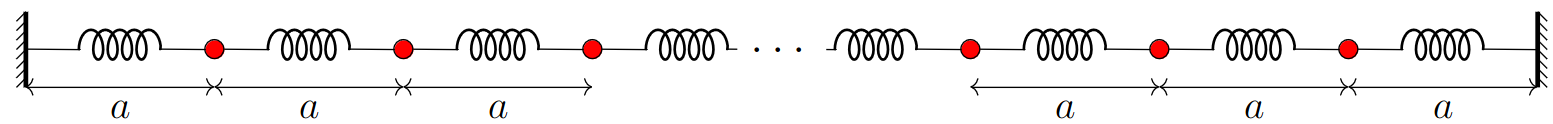
\includegraphics[width = 6.0in]{q1.png}
    \begin{enumerate}[label={(\alph*)}]
        \item Find the equation of the motion of $n^{th}$ bead for the longitudinal mode of vibration
        \item Assuming normal mode vibration, find the normal mode frequency $\omega_m$ for $m^{th}$ mode.
        \item Find the amplitudes of the beads in $m^{th}$ mode ($A^{(m)}_n$ using the notation used in the class).
        \item Plot the dispersion relation $\omega$ versus $k$.
        \item Check whether we have $\omega_{N+2} = \omega_N$?
        \item Check whether we have $A^{(N +2)}_n = A^{(N)}_n$?
        \item Qualitatively plot $A^{(1)}_n$ and $A^{(N)}_n$ for all $n$.
    \end{enumerate}
\end{exercise}
 
\begin{solution}
    $ $
    \begin{enumerate}[label={(\alph*)}]
        \item Let the displacement in the $n^{th}$ bead be $x_n$. Then, for the $n^{th}$ particle we have
        \begin{figure}[h]
            \centering
            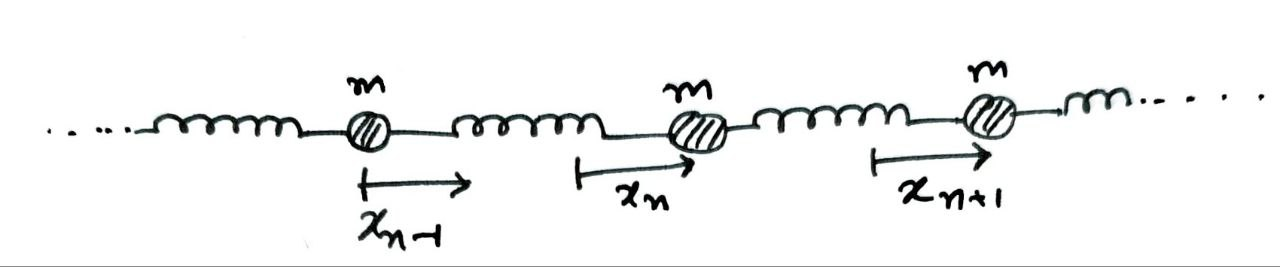
\includegraphics[width = 4.0in]{beaded_string.jpg}
        \end{figure}
            \begin{align*}
                &m\ddot{x_n} = \frac{T}{a}(x_{n-1} - x_n + x_{n+1} - x_n) \\ 
            \Rightarrow &\ddot{x}_n= -\frac{T}{ma}(2x_n - x_{n+1} - x_{n-1})
            \end{align*}
            Let $\omega_0 = \sqrt{\frac{T}{ma}}$. Then, for the $n^{th}$ particle, the equation of motion turns out to be,
            $$\boxed{\ddot{x}_n= -\omega_0^2(2x_n - x_{n+1} - x_{n-1})}$$
        \item Let the amplitude of the $n^{th}$ particle and the frequency in the oscillation in a normal mode be
            be $A_{n}$ and $\omega$ respectively. Then, $x_n = A_n e^{i\omega t}$. So, from the equation of motion we have,
            \begin{align*}
                &\ddot{x}_n = -\omega_0^2(2x_n - x_{n-1} - x_{n + 1}) \\ 
                \Rightarrow & -\omega^2A_n e^{i \omega t} = -\omega_0^2(2A_n e^{i\omega t} - A_{n-1} e^{i\omega t} - A_{n+1} e^{i\omega t}) \\
                \Rightarrow & -\omega^2A_n= -\omega_0^2(2A_n - A_{n-1} - A_{n+1}) \\
                \Rightarrow &\frac{2\omega_0^2 - \omega^2}{\omega_0^2} = \frac{A_{n+1} + A_{n -1}}{A_n} \tag{i}
            \end{align*}
            Observe that, we have a system of $N$ equations, satisfying this relation.
            We claim that for all $\omega \leq 2\omega_0$, the $A_n$'s that satisfy these $N$ equations, can be written as :
            $$A_n = B\cos n\theta + C\sin{n\theta}$$
            where $B,C,\theta$ are constants.
            Now we shall prove this. Observe that 
            \begin{align*}
                \frac{A_{n+1} + A_{n-1}}{A_n} &= \frac{B\cos{(n+1)\theta} + C\cos{(n+1)\theta}+B\cos{(n-1)\theta} + C\cos{(n-1)\theta}}{B\cos{n\theta} + C\cos{n\theta}} \\ 
                                              &=\frac{2B\cos{n\theta}\cos{\theta} + 2C\sin{n\theta}\cos{\theta}}{B\cos{n\theta} + C\sin{n\theta}} \\ 
                                              &=2\cos\theta \tag{ii}
            \end{align*}
            Hence, from equation (i) we have 
            \begin{align*}
                &2\cos\theta = \frac{2\omega_0^2 - \omega^2}{\omega_0^2} \\ 
                \Rightarrow  &\theta = \arccos\left(\frac{2\omega_0^2 - \omega^2}{2\omega_0^2}\right) \tag{iii}
            \end{align*}
            Note that, this equation is valid because $\omega \leq 2\omega_0$.
            Now, $A_0 = B\cos0 + C\sin0 = B$. And $A_1 = B\cos\theta + C\sin\theta \Rightarrow A_1 = A_0\cos\theta + C\sin\theta \Rightarrow C = \frac{A_1 - A_0\cos\theta}{\sin\theta}$
            This uniquely determines $B, C, \text{ and } \theta$. The claim is satisfied for $n=0$ and $n=1$. Now we show inductively that it holds for all $n$.

            Let's say this result holds for all $n \in \{0,\dots,k\}$. Then, from (ii) we have 
            \begin{align*}
                A_{k+1} &= 2A_k\cos\theta = A_{k-1} \\ 
                        &=2B\cos{k\theta}\cos\theta + 2C\sin{k\theta}\cos\theta - B\cos{(k-1)\theta} - C\sin{(k-1)\theta} \\ 
                        &=B\cos{(k+1)\theta} + \cancel{B\cos{(k-1)\theta}} + C\sin{(k+1)\theta} - \cancel{C\sin{(k-1)\theta}}- \cancel{B\cos{(k-1)\theta}} - \cancel{C\sin{(k-1)\theta}} \\ 
                        &=B\cos{(k+1)\theta} + C\sin{(k+1)\theta}
            \end{align*}
            Hence, it holds for $n = k+1$ as well. By the principle of strong induction we can say that the claim holds true for all $n$.
            Now, observe that from (iii) we have, 
            \begin{align*}
                &\frac{2\omega_0^2 - \omega^2}{2\omega_0^2} = \cos\theta \\ 
                \Rightarrow &\omega^2 = 2\omega_0^2(1- \cos\theta) \\ 
                \Rightarrow &\omega^2 = 2\omega_0^2 \cdot 2\sin^2\frac{\theta}{2} \\ 
                \Rightarrow &\omega^2 = 4\omega_0^2\sin^2\frac{\theta}{2} \\
                \Rightarrow &\omega = 2\omega_0\sin\frac{\theta}{2} \tag{iv}
            \end{align*}
            Applying the wall boundary conditions we get 
            $$A_0 = 0 \Rightarrow B\cos0 + C\sin0 = 0 \Rightarrow \boxed{B = 0}$$
            and 
            $$A_{N + 1} = 0 \Rightarrow C\sin{(N + 1)\theta} = 0 \Rightarrow \boxed{\theta = \frac{m\pi}{N + 1}}$$
            where $m \in \nn$. Hence $\theta$ can only take these discrete values as determined by $m$. Hence, $m$ must denote the normal mode. 
            Let $\omega_m$ be the normal mode frequency corresponding to the $m^{th}$ normal mode.
            Then, from (iv) we have,
            $$\boxed{\omega_m = 2\omega_0 \sin{\frac{m\pi}{2(N+1)}}}$$
        \item Also, for the $m^{th}$ normal mode the amplitude of the $n^{th}$ particle
            will be given by,
            $$\boxed{A_n^{( m )} = C\sin{\frac{nm\pi}{N+1}}}$$
        \item 
            In our case of a beaded string, in the $m^{th}$ normal mode, $\lambda = \frac{2L}{m\pi}$. Hence, $k = \frac{m\pi}{(N+1)a}$ Thus, we have 
            $$\boxed{\omega = 2\omega_0\sin{\frac{ka}{2}}}$$
            Hence, the plot for the dispersion relation will be :
            \begin{figure}[h]
                \centering
                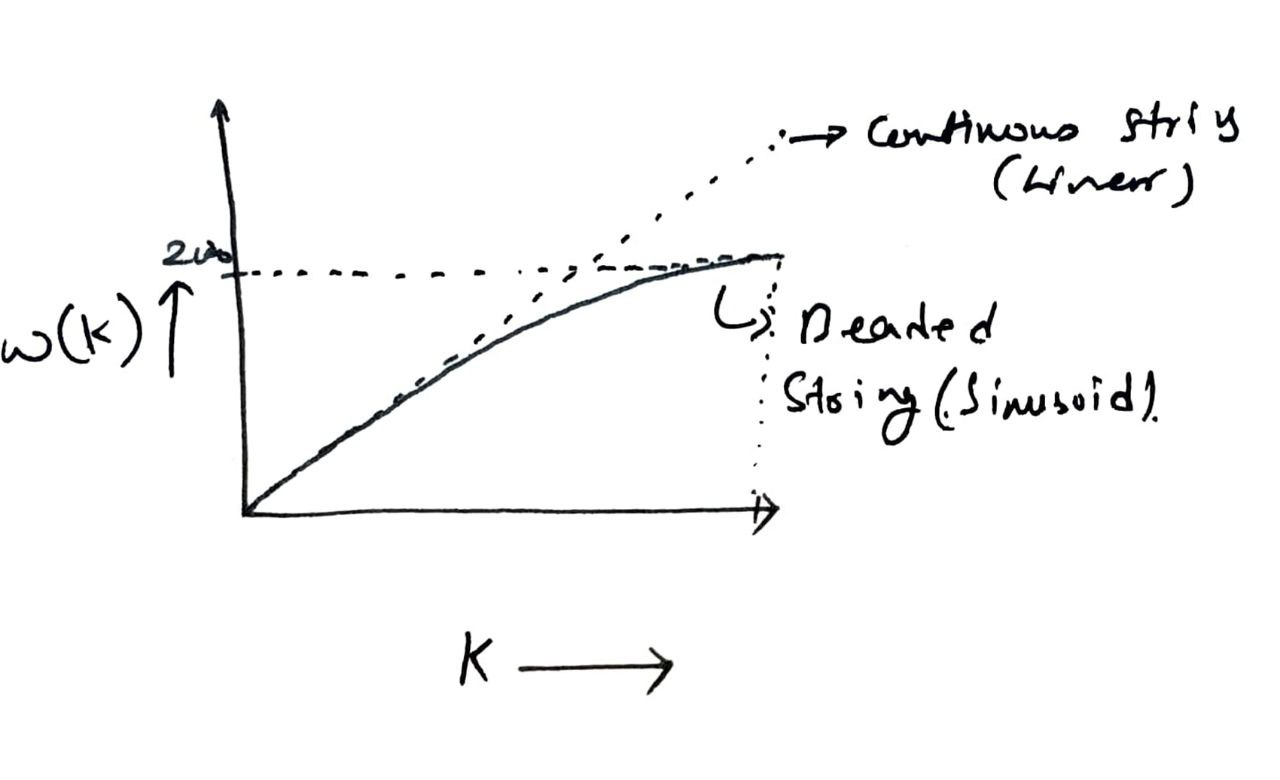
\includegraphics[width=3.0in]{dispersion_relation.jpg}
            \end{figure}
        \item From (b) we have,
            $$\omega_{N+2} = 2\omega_0\sin{\frac{(N+2)\pi}{2(N + 1)}} = 2\omega_0 \sin\frac{(2N + 2 - N)\theta}{2(N + 1)} = 2\omega_0\sin\left(\pi - \frac{N\pi}{2(N + 1)}\right) = \omega_N$$
            Hence, they correspond to the same normal mode.
        \item From (c) we have,
            $$A_{n}^{(N+2)} = C\sin{\frac{n(N+2)\pi}{N + 1}} = C\sin\frac{n(2N + 2 - N)\theta}{N + 1} = C\sin\left(2n\pi - \frac{nN\pi}{N + 1}\right) = -A_n^{(N)}$$
\clearpage
        \item The plot for $A_n^{(1)}$ looks like, 
            \begin{figure}[h]
                \centering
                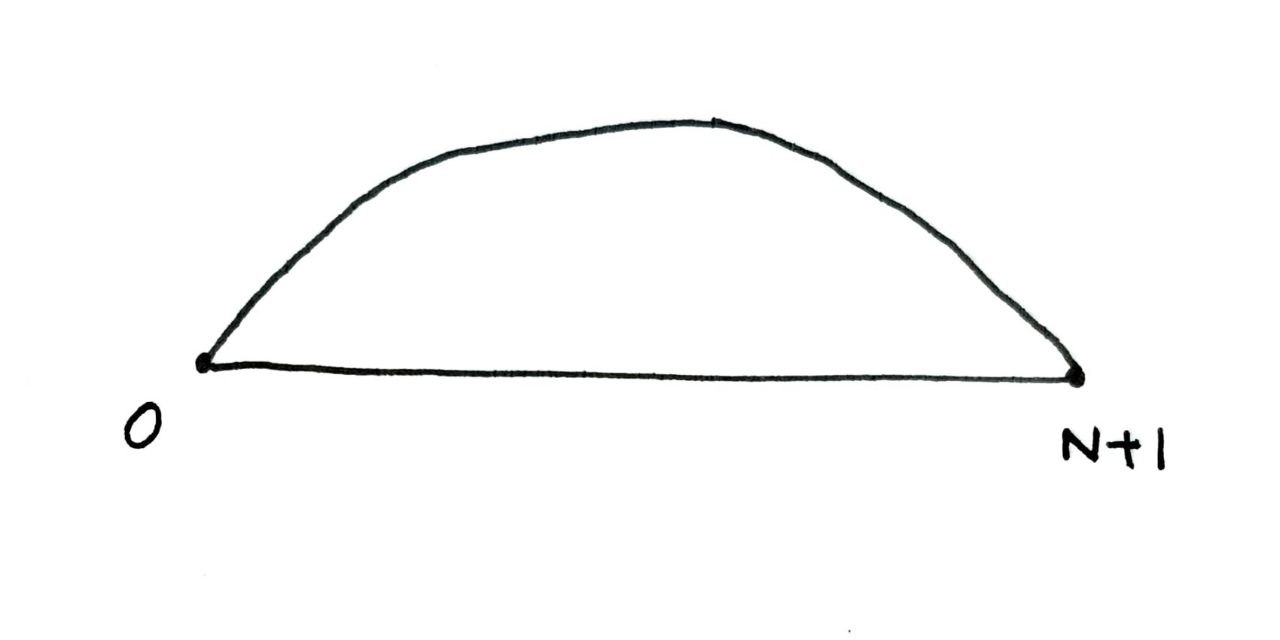
\includegraphics[width=2.0in]{A_1.jpg}
            \end{figure}

            The plot for $A_n^{(N)}$ looks like,
            \begin{figure}[h]
                \centering
                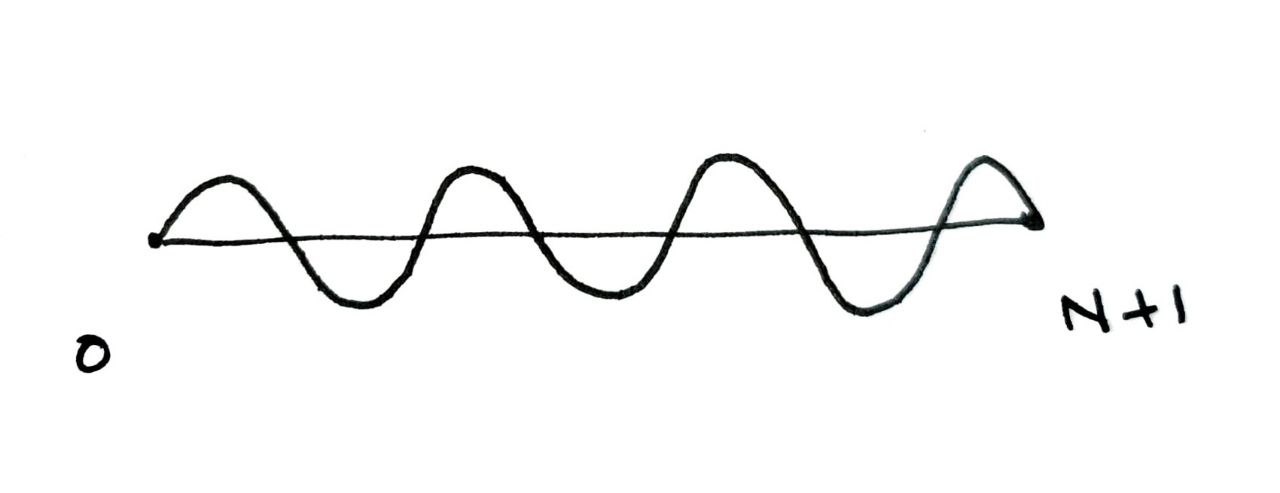
\includegraphics[width=2.0in]{A_n.jpg}
            \end{figure}

            However, the beads will be on the same sinusoidal enevelope as created by the first normal mode. Only the sign will change,
            i.e. the first bead will be on the upper envelope, the second bead will be on the bottom envelope, and so on.
    \end{enumerate}
\end{solution}
\begin{exercise}
    Consider two pendulums, $a$ and $b$, with the same string length $L$, but with different bob masses, $M_a$ and $M_b$. They are coupled by a spring of spring constant $K$ which 
    is attached to the bobs. Assuming small angle oscillations,
    \begin{enumerate}[label={(\alph*)}]
        \item Find the equations of motion using angles of the pendulums (w.r.t. the vertical) as dynamical variables.
        \item Find the normal modes and the normal frequencies.
        \item For $M_a = M_b = M$ does this reduce to the case considered in class?
    \end{enumerate}
\end{exercise}
\begin{solution}
    Let the left and right bobs be given small angular displacements $\theta_1$ and $\theta_2$ respectively, according to the diagram below.
    \begin{figure}[h]
        \centering
        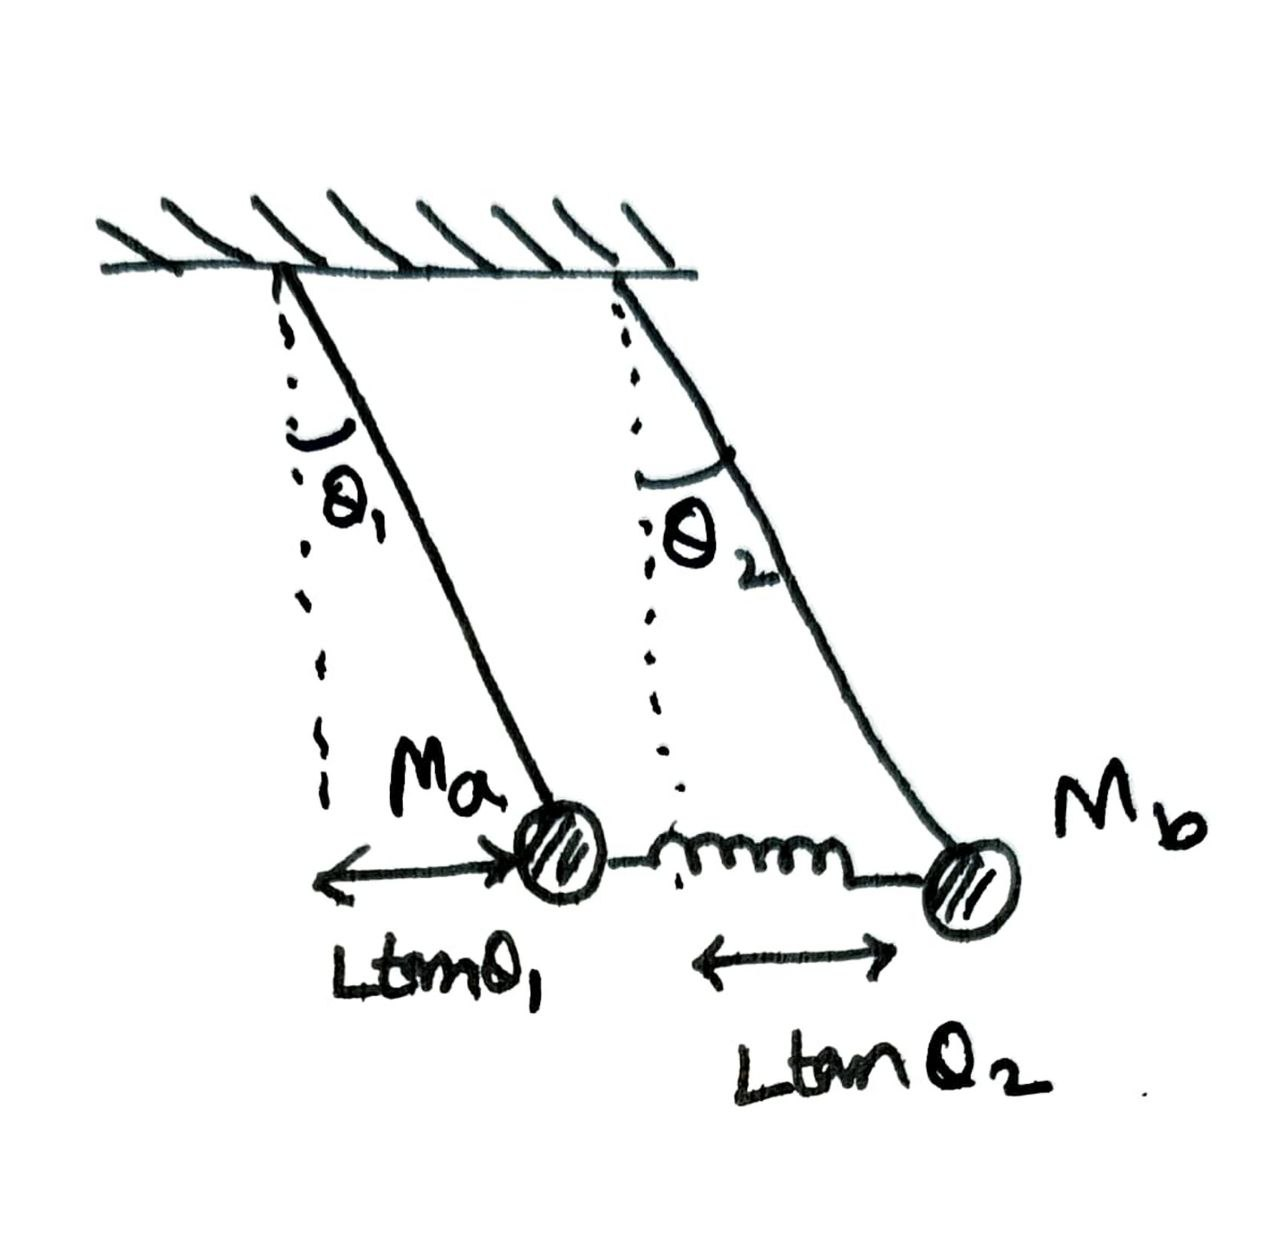
\includegraphics[width=2.0in]{pendulum.jpg}
    \end{figure}
    \begin{enumerate}[label={(\alph*)}]
        \item Then for the left bob we obtain the equation, 
            \begin{align*}
                &\tau = -M_a g \sin\theta_1 - KL^2\tan\theta_1 + KL^2\tan\theta_2 \\ 
                \Rightarrow &I\ddot{\theta_1} = -M_a g L\theta_1 - KL^2\theta_1 + KL^2\theta_2 \\ 
                \Rightarrow &M_a L^2\ddot{\theta_1} = -M_a g L\theta_1 - KL^2(\theta_1 - \theta_2) \\ 
                \Rightarrow &\ddot{\theta_1} = -\frac{g}{L}\theta_1 - \frac{K}{M_a}(\theta_1 -\theta_2)
            \end{align*}
            Similarly, for the right bob we will have, 
            \begin{align*}
                &\tau = -M_b g \sin\theta_2 - KL^2\tan\theta_2 + KL^2\tan\theta_1 \\ 
                \Rightarrow &I\ddot{\theta_2} = -M_b g L\theta_2 - KL^2\theta_2 + KL^2\theta_1 \\ 
                \Rightarrow &M_b L^2\ddot{\theta_2} = -M_b g L\theta_2 - KL^2(\theta_2 - \theta_1) \\ 
                \Rightarrow &\ddot{\theta_2} = -\frac{g}{L}\theta_2 - \frac{K}{M_b}(\theta_2 -\theta_1)
            \end{align*}
            Hence the equations of motion are
            $$\boxed{\ddot{\theta_1} = -\frac{g}{L}\theta_1 - \frac{K}{M_a}(\theta_1 -\theta_2)}$$
            $$\boxed{\ddot{\theta_2} = -\frac{g}{L}\theta_2 - \frac{K}{M_b}(\theta_2 -\theta_1)}$$
        \item Let $\theta_1 = Ae^{i\omega t}$ and $\theta_2 = Be^{i\omega t}$
            Then, we have $\ddot\theta_1 = -\omega^2Ae^{i\omega t}$ and $\theta_2 = -\omega^2 Be^{i\omega t}$

            Putting these values into the equations of motion we get,
            \begin{align*}
                &-\omega^2Ae^{i\omega t} = -\frac{g}{L}Ae^{i \omega t} - \frac{K}{M_a}(Ae^{i \omega t} -Be^{i\omega t}) \\ 
                \Rightarrow &\left(\frac{K}{M_a} + \frac{g}{L} - \omega^2\right)A - \frac{K}{M_a}B = 0
            \end{align*}
            \begin{align*}
                &-\omega^2Be^{i\omega t} = -\frac{g}{L}Be^{i \omega t} - \frac{K}{M_b}(Be^{i \omega t} -Ae^{i\omega t}) \\ 
                \Rightarrow &\left(\frac{K}{M_b} + \frac{g}{L} - \omega^2\right)B - \frac{K}{M_b}A = 0
            \end{align*}
            This system of linear equations can be represented as, 
            \begin{gather*}
                \begin{pmatrix}
                    \left(\frac{K}{M_a} + \frac{g}{L} - \omega^2\right) & -\frac{K}{M_a} \\
                    -\frac{K}{M_b} & \left(\frac{K}{M_b} + \frac{g}{L} - \omega^2\right) 
                \end{pmatrix}
                \begin{pmatrix}
                    A \\ 
                    \\
                    \\
                    B
                \end{pmatrix}
                =
                \begin{pmatrix}
                    0 \\ 
                    \\ 
                    \\
                    0
                \end{pmatrix}
            \end{gather*}
            For this system to have non-trivial solutions, the determinant of the matrix on the left must be 0. Hence,
            \begin{align*}
                &\left(\frac{K}{M_a} + \frac{g}{L} - \omega^2\right)\left(\frac{K}{M_b} + \frac{g}{L} - \omega^2\right) - \frac{K^2}{M_aM_b} = 0 \\ 
                \Rightarrow &\left(\frac{g}{L} - \omega^2\right)^2 + \left(\frac{g}{L} - \omega^2\right)\left(\frac{K}{M_a} + \frac{K}{M_b}\right) = 0 \\
                \Rightarrow &\left(\frac{g}{L} - \omega^2\right)\left[\left(\frac{g}{L} - \omega^2\right)+\left(\frac{K}{M_a} + \frac{K}{M_b}\right)\right] = 0 \\
                \Rightarrow & \omega = \pm \sqrt{\frac{g}{L}} \text{ or, } \omega = \pm \sqrt{\frac{g}{L} + K \left(\frac{1}{M_a} + \frac{1}{M_b}\right)}
            \end{align*}
            We can remove the negative frequencies since they dont give us any new information. Hence we have obtained the normal mode frequencies to be, 
            $$\boxed{\omega =  \sqrt{\frac{g}{L}} \And \sqrt{\frac{g}{L} + K \left(\frac{1}{M_a} + \frac{1}{M_b}\right)}}$$
            In the normal mode corresposing to $\omega = \sqrt{\frac{g}{L}}$, the system of equations gives us
            \begin{align*}
                &\frac{K}{M_a}A - \frac{K}{M_a}B = 0 \And \frac{K}{M_b}B - \frac{K}{M_b}A = 0\\ 
                \Rightarrow &\boxed{A = B}
            \end{align*}
            Hence, in this normal mode, the bobs are oscillating \textbf{in phase}.

            In the normal mode corresposing to $\omega = \sqrt{\frac{g}{L} + K\left(\frac{1}{M_a} + \frac{1}{M_b}\right)}$, the system of equations gives us
            \begin{align*}
                &-\frac{K}{M_b}A - \frac{K}{M_a}B = 0 \And -\frac{K}{M_a}B - \frac{K}{M_b}A = 0\\ 
                \Rightarrow &\boxed{A = -\frac{M_b}{M_a}B}
            \end{align*}
            Hence, in this normal mode, the bobs are oscillating \textbf{out of phase}.
        \item If $M_a = M_b = M$, we get the normal mode frequencies to be
            $$\boxed{\omega =  \sqrt{\frac{g}{L}} \And \sqrt{\frac{g}{L} + \frac{2K}{M}}}$$
            This is similar to thenormal modes obtained for the two mass  coupled osscilator, which were obtained obtained to be, 
            $$\boxed{\omega =  \sqrt{\frac{K_1}{M}} \And \sqrt{\frac{K_1}{M} + \frac{2K_2}{M}}}$$
            In our case, $\frac{g}{L}$ coresponds to the $\frac{K_1}{M}$ in the coupled oscillator.
    \end{enumerate}
\end{solution}
\begin{exercise}
    Consider the following string, with the given configuration

    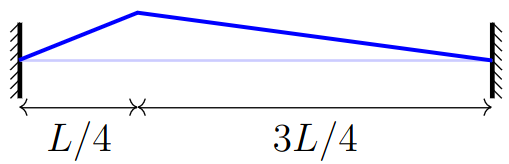
\includegraphics[width = 2.0in]{q2.png}
    \begin{enumerate}[label={(\alph*)}]
        \item Find the fourier representation of the string. You should use the sine representation for the string. (not the full representation).
        \item Show that normal modes having nodes at L/4 are absent.
        \item Check numerically that your solution matches with the given shape. You may submit
        your codes.
    \end{enumerate}
    \begin{solution}
        $ $
        \begin{enumerate}[label={(\alph*)}]
            \item According to the given configuration, 
                \begin{align*}
                    y(x, 0) = 
                    \begin{cases}
                        \frac{4h}{L}x~~~~~~~~~~\text{ for }0<x<\frac{L}{4}\\ 
                        \\
                        \frac{4h}{3L}(L-x)~\,\text{ for }\frac{L}{4}<x<L 
                    \end{cases}
                \end{align*}
                Let the fourier series exapansion of $y(x, 0)$ be
                $$y(x, 0) = \sum_{n=1}^{\infty}c_n \sin \frac{n\pi x}{L}$$
                Then,
                \begin{align*}
                    c_n &=\frac{2}{L} \int_{0}^{L}f(x)\sin\frac{n\pi x}{L}\dx \\ 
                        &= \frac{8h}{L^2}\int_{0}^{\frac{L}{4}}x\sin\npixL \dx + \frac{8h}{3L^2}\int_{\frac{L}{4}}^{L} (L-x)\sin \npixL \dx \\ 
                        &= \frac{8h}{L^2}\left[\int_{0}^{\frac{L}{4}}x\sin\npixL \dx + \frac{1}{3}\int_{\frac{L}{4}}^{L} (L-x)\sin \npixL \dx\right] \\ 
                        &= \frac{8h}{L^2}\left[\int_{0}^{\frac{L}{4}}x\sin\npixL \dx - \frac{1}{3}\int_{\frac{L}{4}}^{L}x\sin \npixL \dx + \frac{1}{3}\int_{\frac{L}{4}}^{L} L\sin\npixL\dx\right] \\ 
                        &= \frac{8h}{L^2}\left[\left(\frac{-Lx}{n\pi}\cos \npixL + \left(\frac{L}{n \pi}\right)^2 \sin \npixL\right)\Big|_{0}^{\frac{L}{4}} -\frac{1}{3}\left(\frac{-Lx}{n\pi}\cos \npixL + \left(\frac{L}{n \pi}\right)^2 \sin \npixL\right)\Big|_{\frac{L}{4}}^{L} - \frac{L^2}{3n\pi} \cos\npixL \Big|_{\frac{L}{4}}^{L}\right] \\
                        &= \frac{8h}{L^2}\left[\left[-\cancel{\frac{L^2}{12n\pi}} + \cancel{\frac{L^2}{3n\pi}} - \cancel{\frac{L^2}{4n\pi}}\right]\cos\frac{n\pi}{4} + \left[-\cancel{\frac{L^2}{3n\pi}}+\cancel{\frac{L^2}{3n\pi}}\right]\cos n\pi + \left(\frac{L}{n\pi}\right)^2\left[1 + \frac{1}{3}\right]\sin \frac{n\pi}{4}\right] \\
                        &= \frac{32h}{3n^2 \pi^2}\sin \frac{n\pi}{4}
                \end{align*}
                Hence, the fourier representation of the string is 
                $$\boxed{y(x,0) = \sum_{n=1}^{\infty}\frac{32h}{3n^2 \pi^2}\sin \frac{n\pi}{4} \sin\npixL}$$
            \item For the normal modes with a node at $x = \frac{L}{4}$ we have, $\sin\npixL = \sin \frac{n\pi}{4}= 0 \Rightarrow n = 4k$ for some $k \in \nn$.
                But, we also have 
                $$\boxed{c_{4k} = \frac{32h}{3\cdot16k^2\cdot\pi^2}\sin\frac{\cancel{4}k\pi}{\cancel{4}} = 0}$$
                Hence, those normal modes are absent in the fourier representation of the string.
            \item 
    Below is a plot of increasing partial sums of the fourier series expansion of the given function

    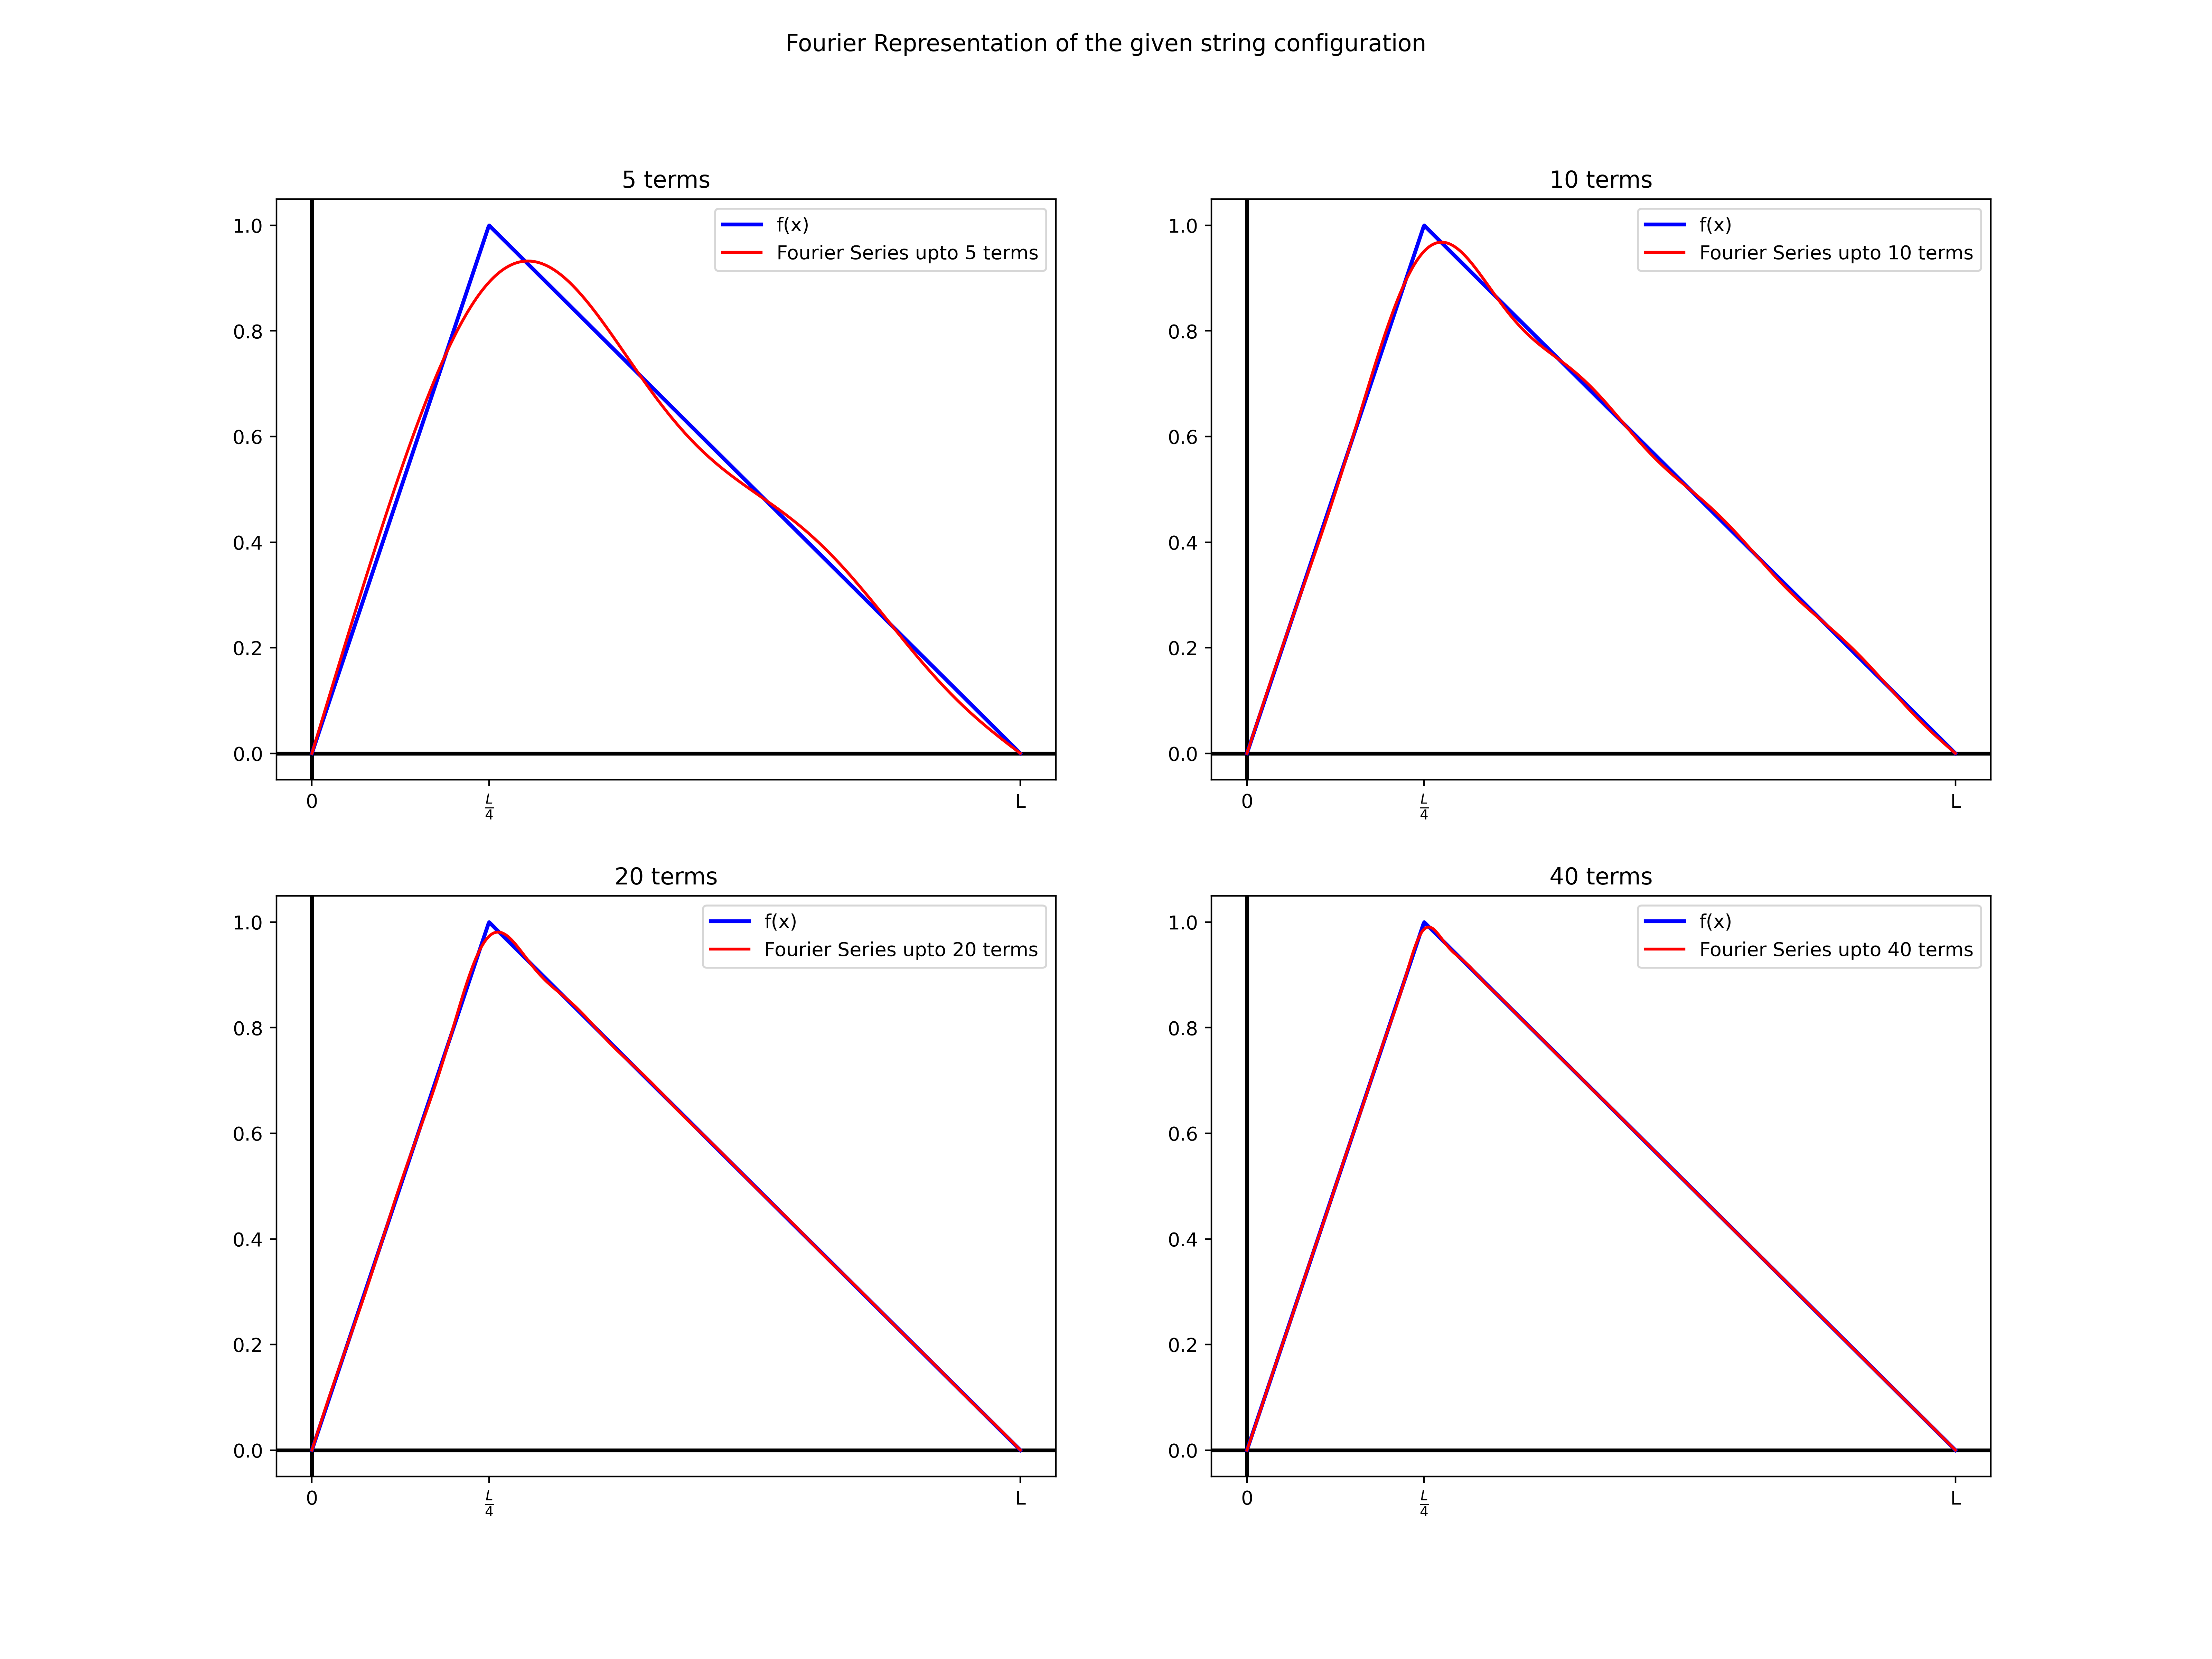
\includegraphics[width = 5.0in]{fourier_series_1.png}

    Here's the code used for generating the above plots :

    \lstinputlisting[language=Python]{fourier1.py}
        \end{enumerate}
    \end{solution}
\end{exercise}
\begin{exercise}
    Consider the following pattern. Find the Fourier representation of this pattern. Use the
    complete representation (using sine and cosine). Also, check numerically that your solution
    matches with the given shape. You may submit your codes.

    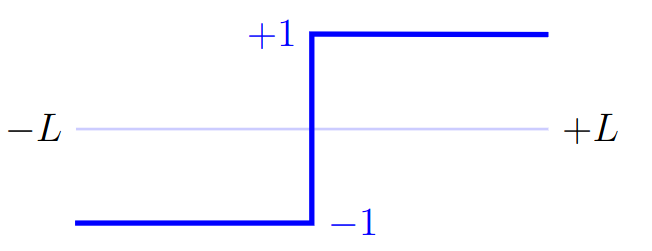
\includegraphics[width = 2.0in]{q3.png}
\end{exercise}
\begin{solution}
    Let the fourier series exapansion of $f(x)$ be, $$f(x) = a_0 + \sum_{n=1}^{\infty}\left(a_n \cos \frac{n\pi x}{L} + b_n \cos \frac{n\pi x}{L}\right)$$

    Then, 
    \begin{align*}
        a_0 &= \frac{1}{2L}\int_{-L}^{L}f(x)\dx = 0
    \end{align*}
    Also, 
    \begin{align*}
        a_n &= \frac{1}{L} \int_{-L}^{L}f(x)\cos\frac{n\pi x}{L}\dx \\
            &= -\frac{1}{L} \int_{-L}^{0} \cos \npixL \dx + \frac{1}{L} \int_{0}^{L}\cos \npixL \dx\\
            &= \frac{1}{L} \int_{0}^{-L} \cos \npixL \dx + \frac{1}{L} \int_{0}^{L}\cos \npixL \dx\\
            &= -\cancel{\frac{1}{L} \int_{0}^{L} \cos \npixL \dx} + \cancel{\frac{1}{L} \int_{0}^{L}\cos \npixL \dx}\\
            &= 0
    \end{align*}
    and,
    \begin{align*}
        b_n &=\frac{1}{L} \int_{-L}^{L}f(x)\sin\frac{n\pi x}{L}\dx \\
            &= -\frac{1}{L}\int_{-L}^{0} \sin \npixL \dx + \frac{1}{L}\int_{0}^{L}\sin \npixL \dx\\
            &= \frac{1}{L}\int_{0}^{-L} \sin \npixL \dx + \frac{1}{L}\int_{0}^{L}\sin \npixL \dx\\
            &= \frac{1}{L}\int_{0}^{L} \sin \npixL \dx + \frac{1}{L}\int_{0}^{L}\sin \npixL \dx\\
            &= 2\frac{1}{L}\int_{0}^{L} \sin \npixL \dx\\
            &= -\frac{1}{\cancel{L}} \cdot \frac{2\cancel{L}}{n\pi}\cos \npixL \dx\Big|_{0}^{L} \\
            &= -\frac{2}{n\pi}(\cos n \pi -1)\\
            &= 
            \begin{cases}
                \frac{4}{n\pi} ~~\text{ if $n$ is odd}\\ 
                0 ~~~~~\text{ if $n$ is even}
            \end{cases}
    \end{align*}
    Hence we have
    $$f(x) = \sum_{n \text{ is odd}}^{\infty} \frac{4}{n\pi}\sin\npixL = \sum_{n=1}^{\infty}\frac{4}{(2n -1)\pi} \sin \frac{(2n -1)\pi x}{L}$$
    Hence, the fourier series exapansion for the given $f(x)$ is 
    $$\boxed{f(x) = \sum_{n=1}^{\infty}\frac{4}{(2n -1)\pi} \sin \frac{(2n -1)\pi x}{L}}$$

    Below is a plot of increasing partial sums of the fourier series expansion of the given function

    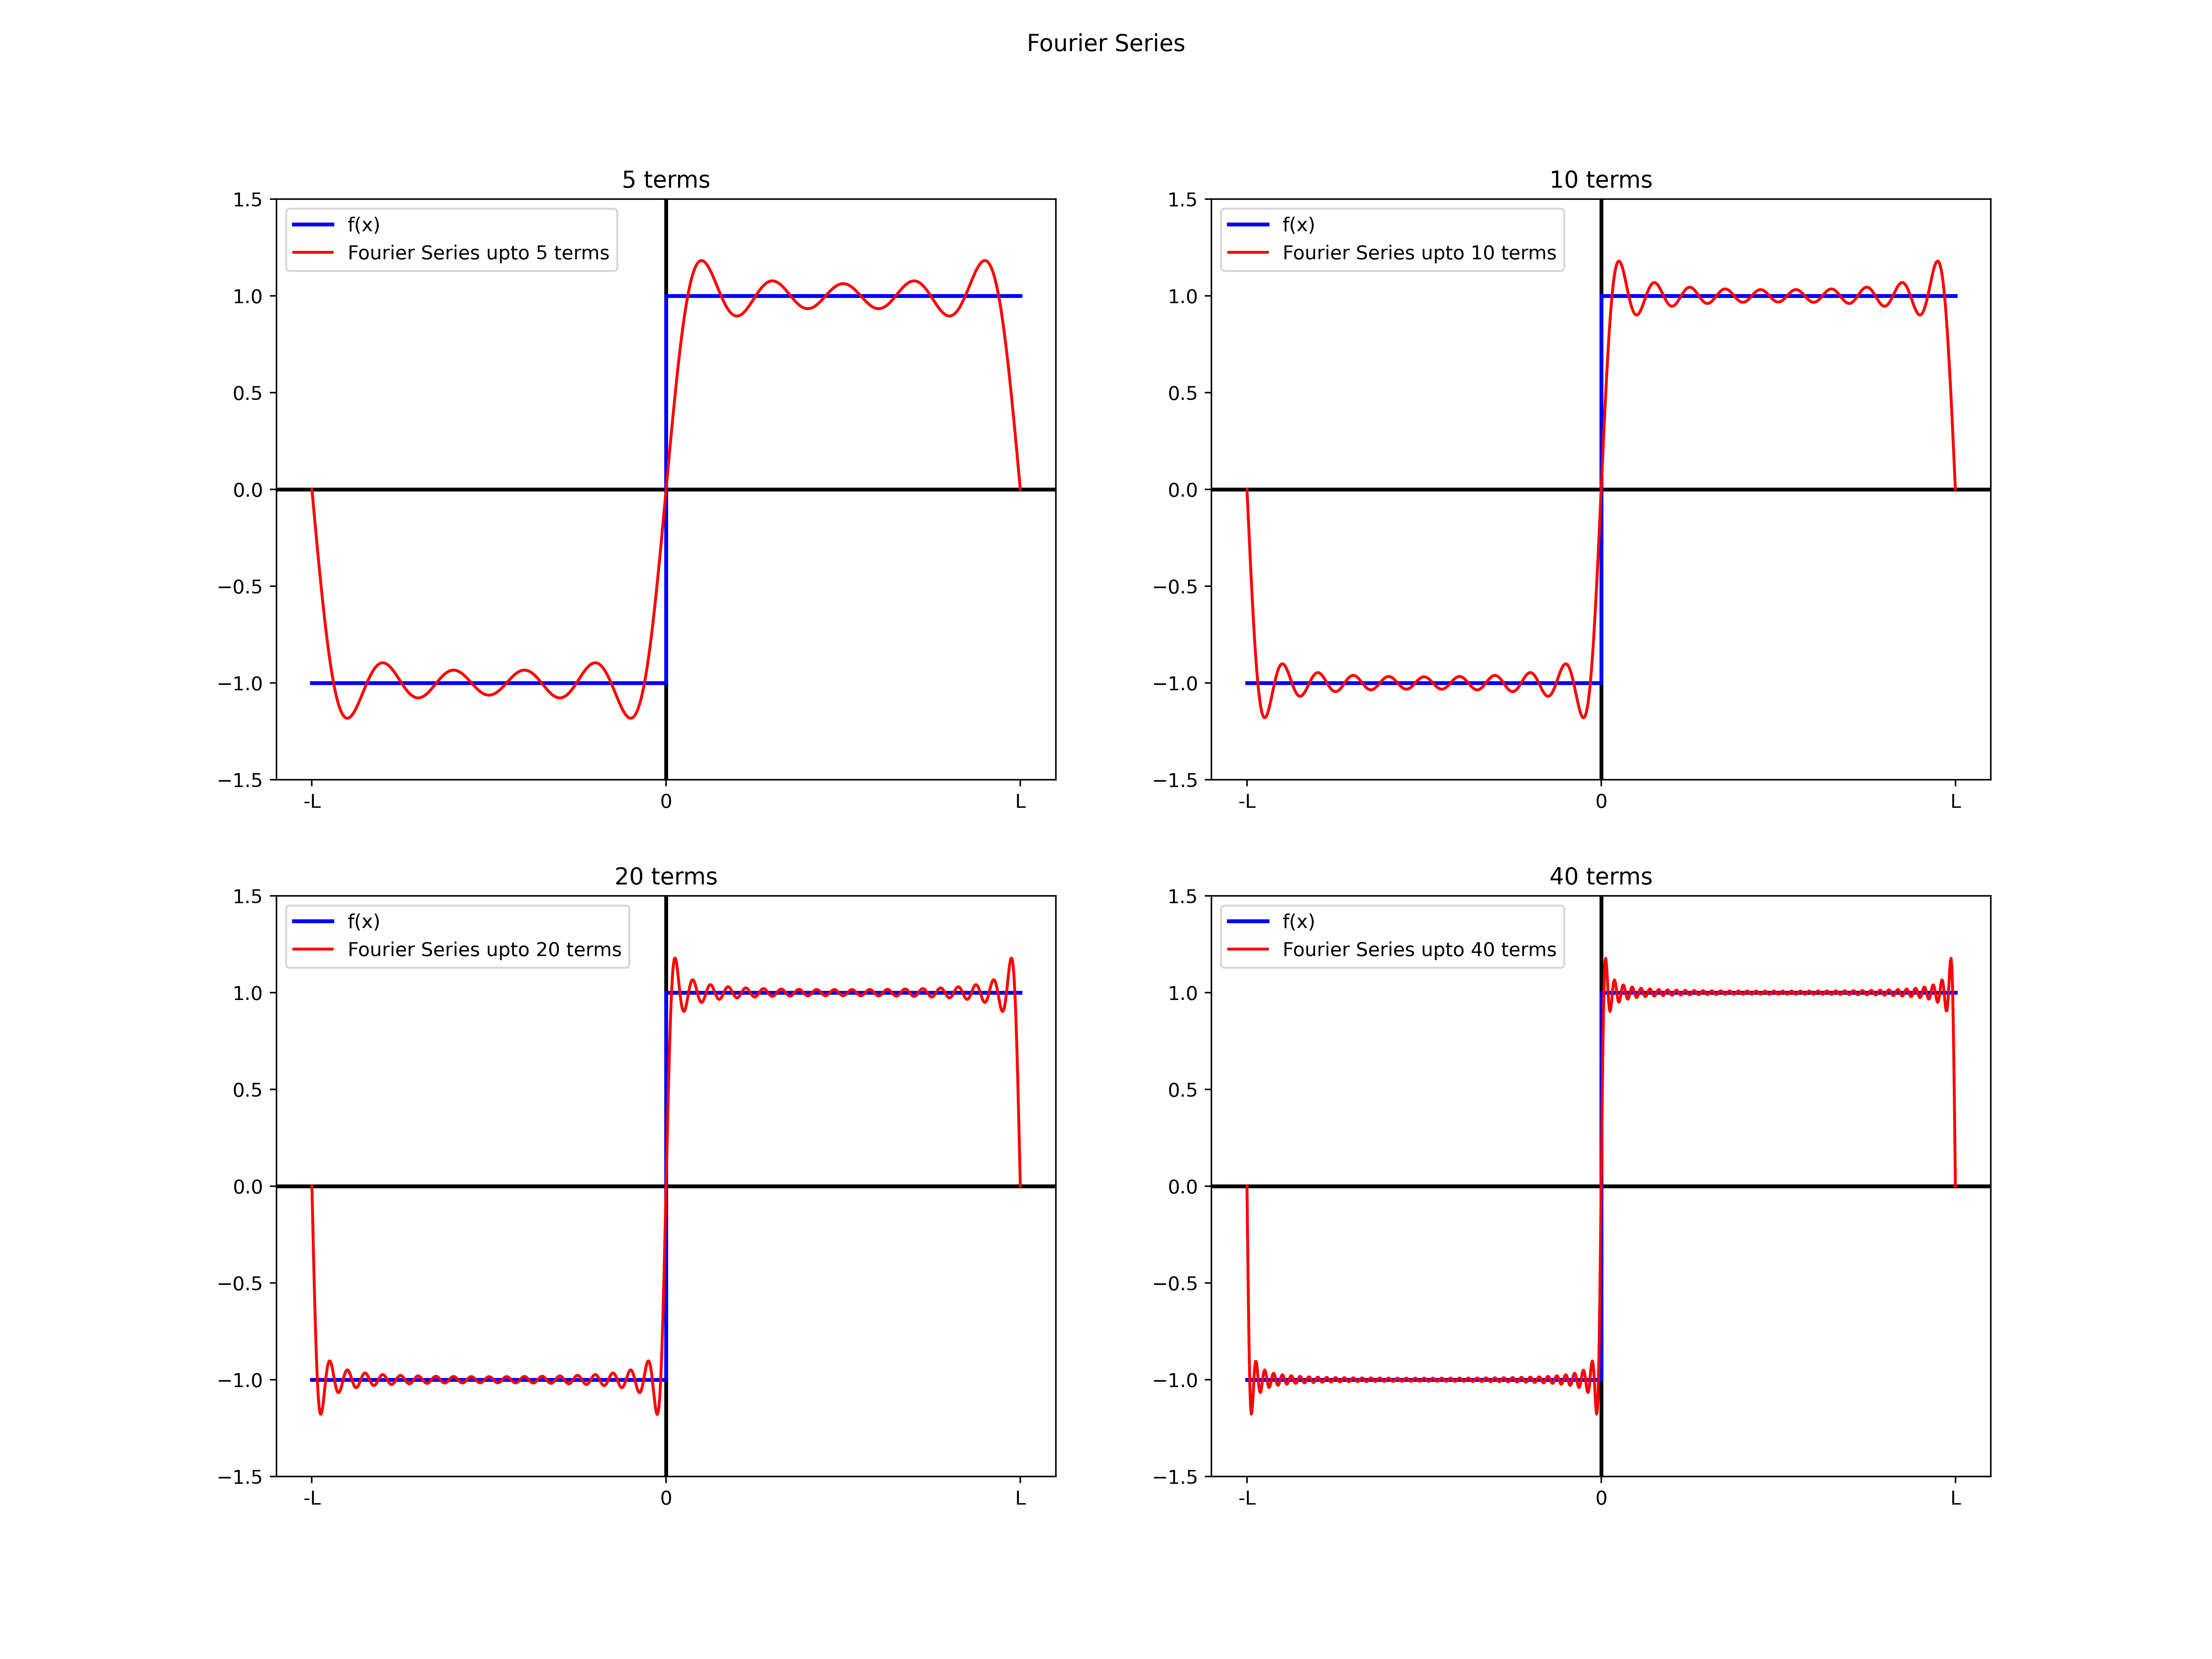
\includegraphics[width = 6.0in]{fourier_series_2.png}

    Here's the code used for generating the above plots :

    \lstinputlisting[language=Python]{fourier2.py}
\end{solution}
\end{document}

